\documentclass[tikz]{standalone}

\usepackage{amsfonts}
\usepackage{amsmath}
\usepackage{braket}

\usepackage{tikz}
\usetikzlibrary{shapes.geometric,patterns,positioning,matrix}
\usetikzlibrary{shadows,calc,3d,arrows.meta,decorations.pathmorphing,decorations.markings,decorations.pathreplacing}

\definecolor{googleB}{HTML}{4285F4}
\definecolor{googleG}{HTML}{34A853}
\definecolor{googleY}{HTML}{FBBC05}
\definecolor{googleR}{HTML}{EA4335}
\definecolor{googleBG}{HTML}{3B96A4}

% load TikZ grafic definitions
%\input{gfx_TikZ}

% main document
\begin{document}
	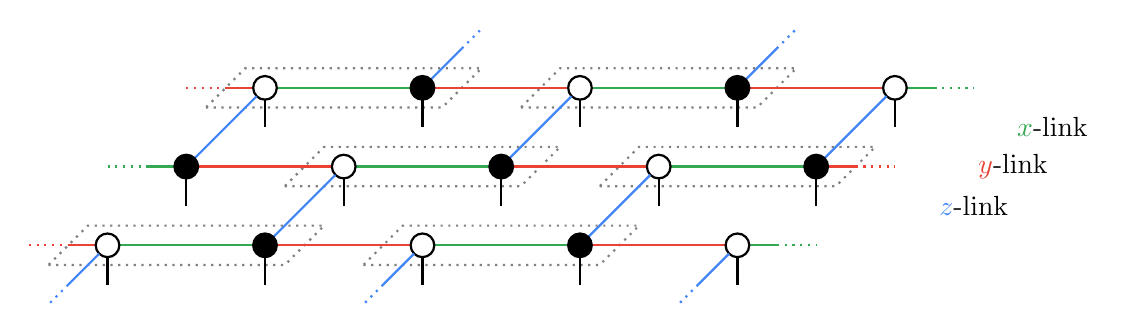
\begin{tikzpicture}

		\def\colorX{googleG}
		\def\colorY{googleR}
		\def\colorZ{googleB}

		\begin{scope}[shift = {(+1.5, +1.5)}]
			\foreach \x in {-2, +2} {
				\draw[thick, \colorZ, shift = {(\x, 0)}, rotate = 45] (-{sqrt(2)/2 - 0.15}, 0) to (0, 0);
				\draw[thick, \colorZ, shift = {(\x, 0)}, rotate = 45, dotted] (0, 0) to (+{sqrt(2)/4}, 0);
			}
			% \foreach \x in {-4, 0, +4} {
			% 	\draw[thick, gray, shift = {(\x, 0)}, rotate = 45, dotted] (-{sqrt(2)/2 - 0.15}, 0) to (+{sqrt(2)/4}, 0);
			% }
		\end{scope}

		\begin{scope}[shift = {(+1, +1)}]
			\begin{scope}[shift = {(-4, 0)}]
				\draw[thick, \colorY, dotted] (-1.0, 0) to (-0.5, 0);
				\draw[thick, \colorY] (-0.5, 0) to (-0.0, 0);
			\end{scope}
			\foreach \x in {-3, +1} {
				\draw[thick, \colorX, shift = {(\x, 0)}] (-0.85, 0) to (+0.85, 0);
				\draw[thick, gray, dotted, shift = {(\x, 0)}] (-1.75, -0.25) to (+1.25, -0.25) to (+1.75, +0.25) to (-1.25, +0.25) -- cycle;
			}
			\foreach \x in {-1, +3} {
				\draw[thick, \colorY, shift = {(\x, 0)}] (-0.85, 0) to (+0.85, 0);
			}
			\begin{scope}[shift = {(+4, 0)}]
				\draw[thick, \colorX] (+0.0, 0) to (+0.5, 0);
				\draw[thick, \colorX, dotted] (+0.5, 0) to (+1.0, 0);
			\end{scope}

			\foreach \x in {-4, 0, +4} {
				\draw[thick] (\x,0) to (\x, -0.5);
				\draw[thick, black, fill = white] (\x, 0) circle (0.15);
			}
			\foreach \x in {-2, +2} {
				\draw[thick] (\x,0) to (\x, -0.5);
				\draw[thick, black, fill = black] (\x, 0) circle (0.15);
			}
		\end{scope}

		\begin{scope}[shift = {(+0.5, +0.5)}]
			\foreach \x in {-4, 0, +4} {
				\draw[thick, \colorZ, shift = {(\x, 0)}, rotate = 45] (-{sqrt(2)/2 - 0.15}, 0) to (+{sqrt(2)/2 - 0.15}, 0);
			}
			% \foreach \x in {-2, +2} {
			% 	\draw[thick, gray, shift = {(\x, 0)}, rotate = 45, dotted] (-{sqrt(2)/2 - 0.15}, 0) to (+{sqrt(2)/2 - 0.15}, 0);
			% }
		\end{scope}

		\begin{scope}[shift = {(0, 0)}]
			\begin{scope}[shift = {(-4, 0)}]
				\draw[thick, \colorX, dotted] (-1.0, 0) to (-0.5, 0);
				\draw[thick, \colorX] (-0.5, 0) to (-0.0, 0);
			\end{scope}
			\foreach \x in {-1, +3} {
				\draw[thick, \colorX, shift = {(\x, 0)}] (-0.85, 0) to (+0.85, 0);
				\draw[thick, gray, dotted, shift = {(\x, 0)}] (-1.75, -0.25) to (+1.25, -0.25) to (+1.75, +0.25) to (-1.25, +0.25) -- cycle;
			}
			\foreach \x in {-3, +1} {
				\draw[thick, \colorY, shift = {(\x, 0)}] (-0.85, 0) to (+0.85, 0);
			}
			\begin{scope}[shift = {(+4, 0)}]
				\draw[thick, \colorY] (+0.0, 0) to (+0.5, 0);
				\draw[thick, \colorY, dotted] (+0.5, 0) to (+1.0, 0);
			\end{scope}

			\foreach \x in {-2, +2} {
				\draw[thick] (\x,0) to (\x, -0.5);
				\draw[thick, black, fill = white] (\x, 0) circle (0.15);
			}
			\foreach \x in {-4, 0, +4} {
				\draw[thick] (\x,0) to (\x, -0.5);
				\draw[thick, black, fill = black] (\x, 0) circle (0.15);
			}
		\end{scope}

		\begin{scope}[shift = {(-0.5, -0.5)}]
			\foreach \x in {-2, +2} {
				\draw[thick, \colorZ, shift = {(\x, 0)}, rotate = 45] (-{sqrt(2)/2 - 0.15}, 0) to (+{sqrt(2)/2 - 0.15}, 0);
			}
			% \foreach \x in {-4, 0, +4} {
			% 	\draw[thick, gray, shift = {(\x, 0)}, rotate = 45, dotted] (-{sqrt(2)/2 - 0.15}, 0) to (+{sqrt(2)/2 - 0.15}, 0);
			% }
		\end{scope}

		\begin{scope}[shift = {(-1, -1)}]
			\begin{scope}[shift = {(-4, 0)}]
				\draw[thick, \colorY, dotted] (-1.0, 0) to (-0.5, 0);
				\draw[thick, \colorY] (-0.5, 0) to (-0.0, 0);
			\end{scope}
			\foreach \x in {-3, +1} {
				\draw[thick, \colorX, shift = {(\x, 0)}] (-0.85, 0) to (+0.85, 0);
				\draw[thick, gray, dotted, shift = {(\x, 0)}] (-1.75, -0.25) to (+1.25, -0.25) to (+1.75, +0.25) to (-1.25, +0.25) -- cycle;
			}
			\foreach \x in {-1, +3} {
				\draw[thick, \colorY, shift = {(\x, 0)}] (-1.0, 0) to (+1.0, 0);
			}
			\begin{scope}[shift = {(+4, 0)}]
				\draw[thick, \colorX] (+0.0, 0) to (+0.5, 0);
				\draw[thick, \colorX, dotted] (+0.5, 0) to (+1.0, 0);
			\end{scope}

			\foreach \x in {-4, 0, +4} {
				\draw[thick] (\x,0) to (\x, -0.5);
				\draw[thick, black, fill = white] (\x, 0) circle (0.15);
			}
			\foreach \x in {-2, +2} {
				\draw[thick] (\x,0) to (\x, -0.5);
				\draw[thick, black, fill = black] (\x, 0) circle (0.15);
			}
		\end{scope}

		\begin{scope}[shift = {(-1.5, -1.5)}]
			\foreach \x in {-4, 0, +4} {
				\draw[thick, \colorZ, shift = {(\x, 0)}, rotate = 45] (0, 0) to (+{sqrt(2)/2 - 0.15}, 0);
				\draw[thick, \colorZ, shift = {(\x, 0)}, rotate = 45, dotted] (0, 0) to (-{sqrt(2)/4}, 0);
			}
			% \foreach \x in {-2, +2} {
			% 	\draw[thick, gray, shift = {(\x, 0)}, rotate = 45, dotted] (-{sqrt(2)/4}, 0) to (+{sqrt(2)/2 - 0.15}, 0);
			% }
		\end{scope}

		\node at (+7.0, +0.5) {{\color{\colorX}$x$}-link};
		\node at (+6.5, +0.0) {{\color{\colorY}$y$}-link};
		\node at (+6.0, -0.5) {{\color{\colorZ}$z$}-link};


      \end{tikzpicture}

\end{document}

%%% Local Variables:
%%% mode: latex
%%% TeX-master: t
%%% End:
